\chapter{Thessa tool}
{
	"\textit{It was born after have face a problem with the generation of a parallel code for the LIM architecture due to the difficulties to detect the data/control dependency without a proper analysis and optimization. This tool allows to be able to generate a parallel code in order to take the most from a multi-core architecture like the LIM.}"
	\\[5pt]
	\rightline{{\rm --- CETRULO E. \cite{tessa}}} \\
 
 It's a tool that given a C code, it translates it into a Mid-level Intermediate Representation code (MIRcode). After that the tool can show the Program Dependence Graph (PDG), the  Control Flow Graph (CFG) and the Quotient graph (Q) of the program in MIRcode. 
\section{Analysis of Thessa on the Binomial filter algorithm}

The binomial filter implemented in this tools, is different from the one in this thesis.
The difference is that in this case it performs an arithmetic average as you can see below in C code (mine was a weighted average)
\lstset{ %Formatting for code in appendix
	language=C,
	basicstyle=\footnotesize,
	numbers=left,
	stepnumber=1,
	showstringspaces=false,
	tabsize=1,
	breaklines=true,
	breakatwhitespace=false,
}

\begin{lstlisting}[frame=single]  % Start your 

#include <stdio.h>
#define V 10000

int main(){
int w = 8;
int h = 8;
int in[h][w] = {{ 0,0,0,0,0,0,0,0},{ 0,1,6,6,1,1,1,0},{ 0,1,6,6,1,1,1,0},{ 0,1,6,6,1,1,1,0},{ 0,1,6,6,1,1,1,0},{ 0,1,6,6,1,1,6,0},{ 0,1,6,6,1,1,6,0},{ 0,0,0,0,0,0,0,0}};
int out[h][w];
int i;
int j;
int divisor = 8;

for (i = 1; i < h-1; i++){
for (j = 1; j < w-1; j=j+1){

out[i][j] = (in[i-1][j-1] + in[i-1][j] + in[i-1][j+1] + in[i][j-1] + in[i][j] + in[i][j+1] + in[i+1][j-1] + in[i+1][j] + in[i+1][j+1])/divisor;
}
}

return 0;
}
\end{lstlisting}
\subsection{Output generated}
\subsubsection{MIRcode}
Having the C code, we have yo translate it in a lower language as the MiRcode and obtain the following code.\\
\begin{tabular}{l l l}
0   & &    ['\$s', 'i', '1'] \\
1     & &  ['+', '\_f1', 'i', '1']\\ 
2 & &      ['-', '\_f0', 'i', '1'] \\
3  & L3:& ['for', '$>$=', 'i', '7', 'goto', 'L0']\\ 
4 & &      ['\$s', 'j', '1'] \\
5    & &   ['+', '\_f3', 'j', '1'] \\
6       & &['-', '\_f2', 'j', '1'] \\
7   &L2:& ['for', '$>$=', 'j', '7', 'goto', 'L1'] \\
8   & &    ['+', '\_t0', 'in[i-1][j]', 'in[i-1][j-1]'] \\
9  & &     ['+', '\_t1', '\_t0', 'in[i-1][j+1]'] \\
10    & &  ['+', '\_t2', '\_t1', 'in[i][j-1]']\\
11& &   ['+', '\_t3', '\_t2', 'in[i][j]']\\
\end{tabular}\\
\begin{tabular}{l l l}
12& &   ['+', '\_t4', '\_t3', 'in[i][j+1]']\\
13& &   ['+', '\_t5', '\_t4', 'in[i+1][j-1]']\\
14& &   ['+', '\_t6', '\_t5', 'in[i+1][j]']\\
15 & &  ['+', '\_t7', '\_t6', 'in[i+1][j+1]']\\ 
16 & &  ['/', '\_t8', '\_t7', 'divisor'] \\
17 & &  ['\$s', 'out[i][j]', '\_t8'] \\
18 & &  ['+', '\_t9', 'j', '1'] \\
19 & &  ['\$s', 'j', '\_t9'] \\
20 & &  ['+', '\_f3', 'j', '1']\\
21 & &  ['-', '\_f2', 'j', '1'] \\
22 & &  ['goto', 'L2']\\
%\end{tabular}\\
%\begin{tabular}{l l l}
23  &L1:& ['+', '\_t10', 'i', '1']\\
24 & &  ['\$s', 'i', '\_t10'] \\
25 & &  ['+', '\_f1', 'i', '1']\\
26 & &  ['-', '\_f0', 'i', '1']\\
27 & &  ['goto', 'L3']\\
28  &L0:& ['\$s', 'reset', '0']\\

\end{tabular}\\
\subsubsection{Program Dependence Graph (PDG)}
After the generation of the MIRcode, we have to understand the data and memory dependencies between each single instruction or some critical sections.
We obtain the following graph (Program Dependence Graph (PDG)) where each number represent a single instruction (as you can see in the previous MiRcode).\\

 This graph is used to recognize the point in the code where it's not possible to parallelize the code. This point are highlighted by the SSCs component that in the figure are colored in gray box. This graph has also a different color and shape edge.\\
  Here we will list all the different color and their meaning: 
  \begin{itemize}
   \item Blue edge : Memory Output Dependence
   \item Red edge : Register Flow Dependence 
   \item Light Green edge : Memory Flow Dependence  
   \item Black edge : Memory Anti-Dependence
   \item Brown dashed edge : Data Dependence with indexes involved 
   \item Dark Green dotted edge : Control Dependence 
  \end{itemize}
  \begin{figure}[h!]
  	\centering
  	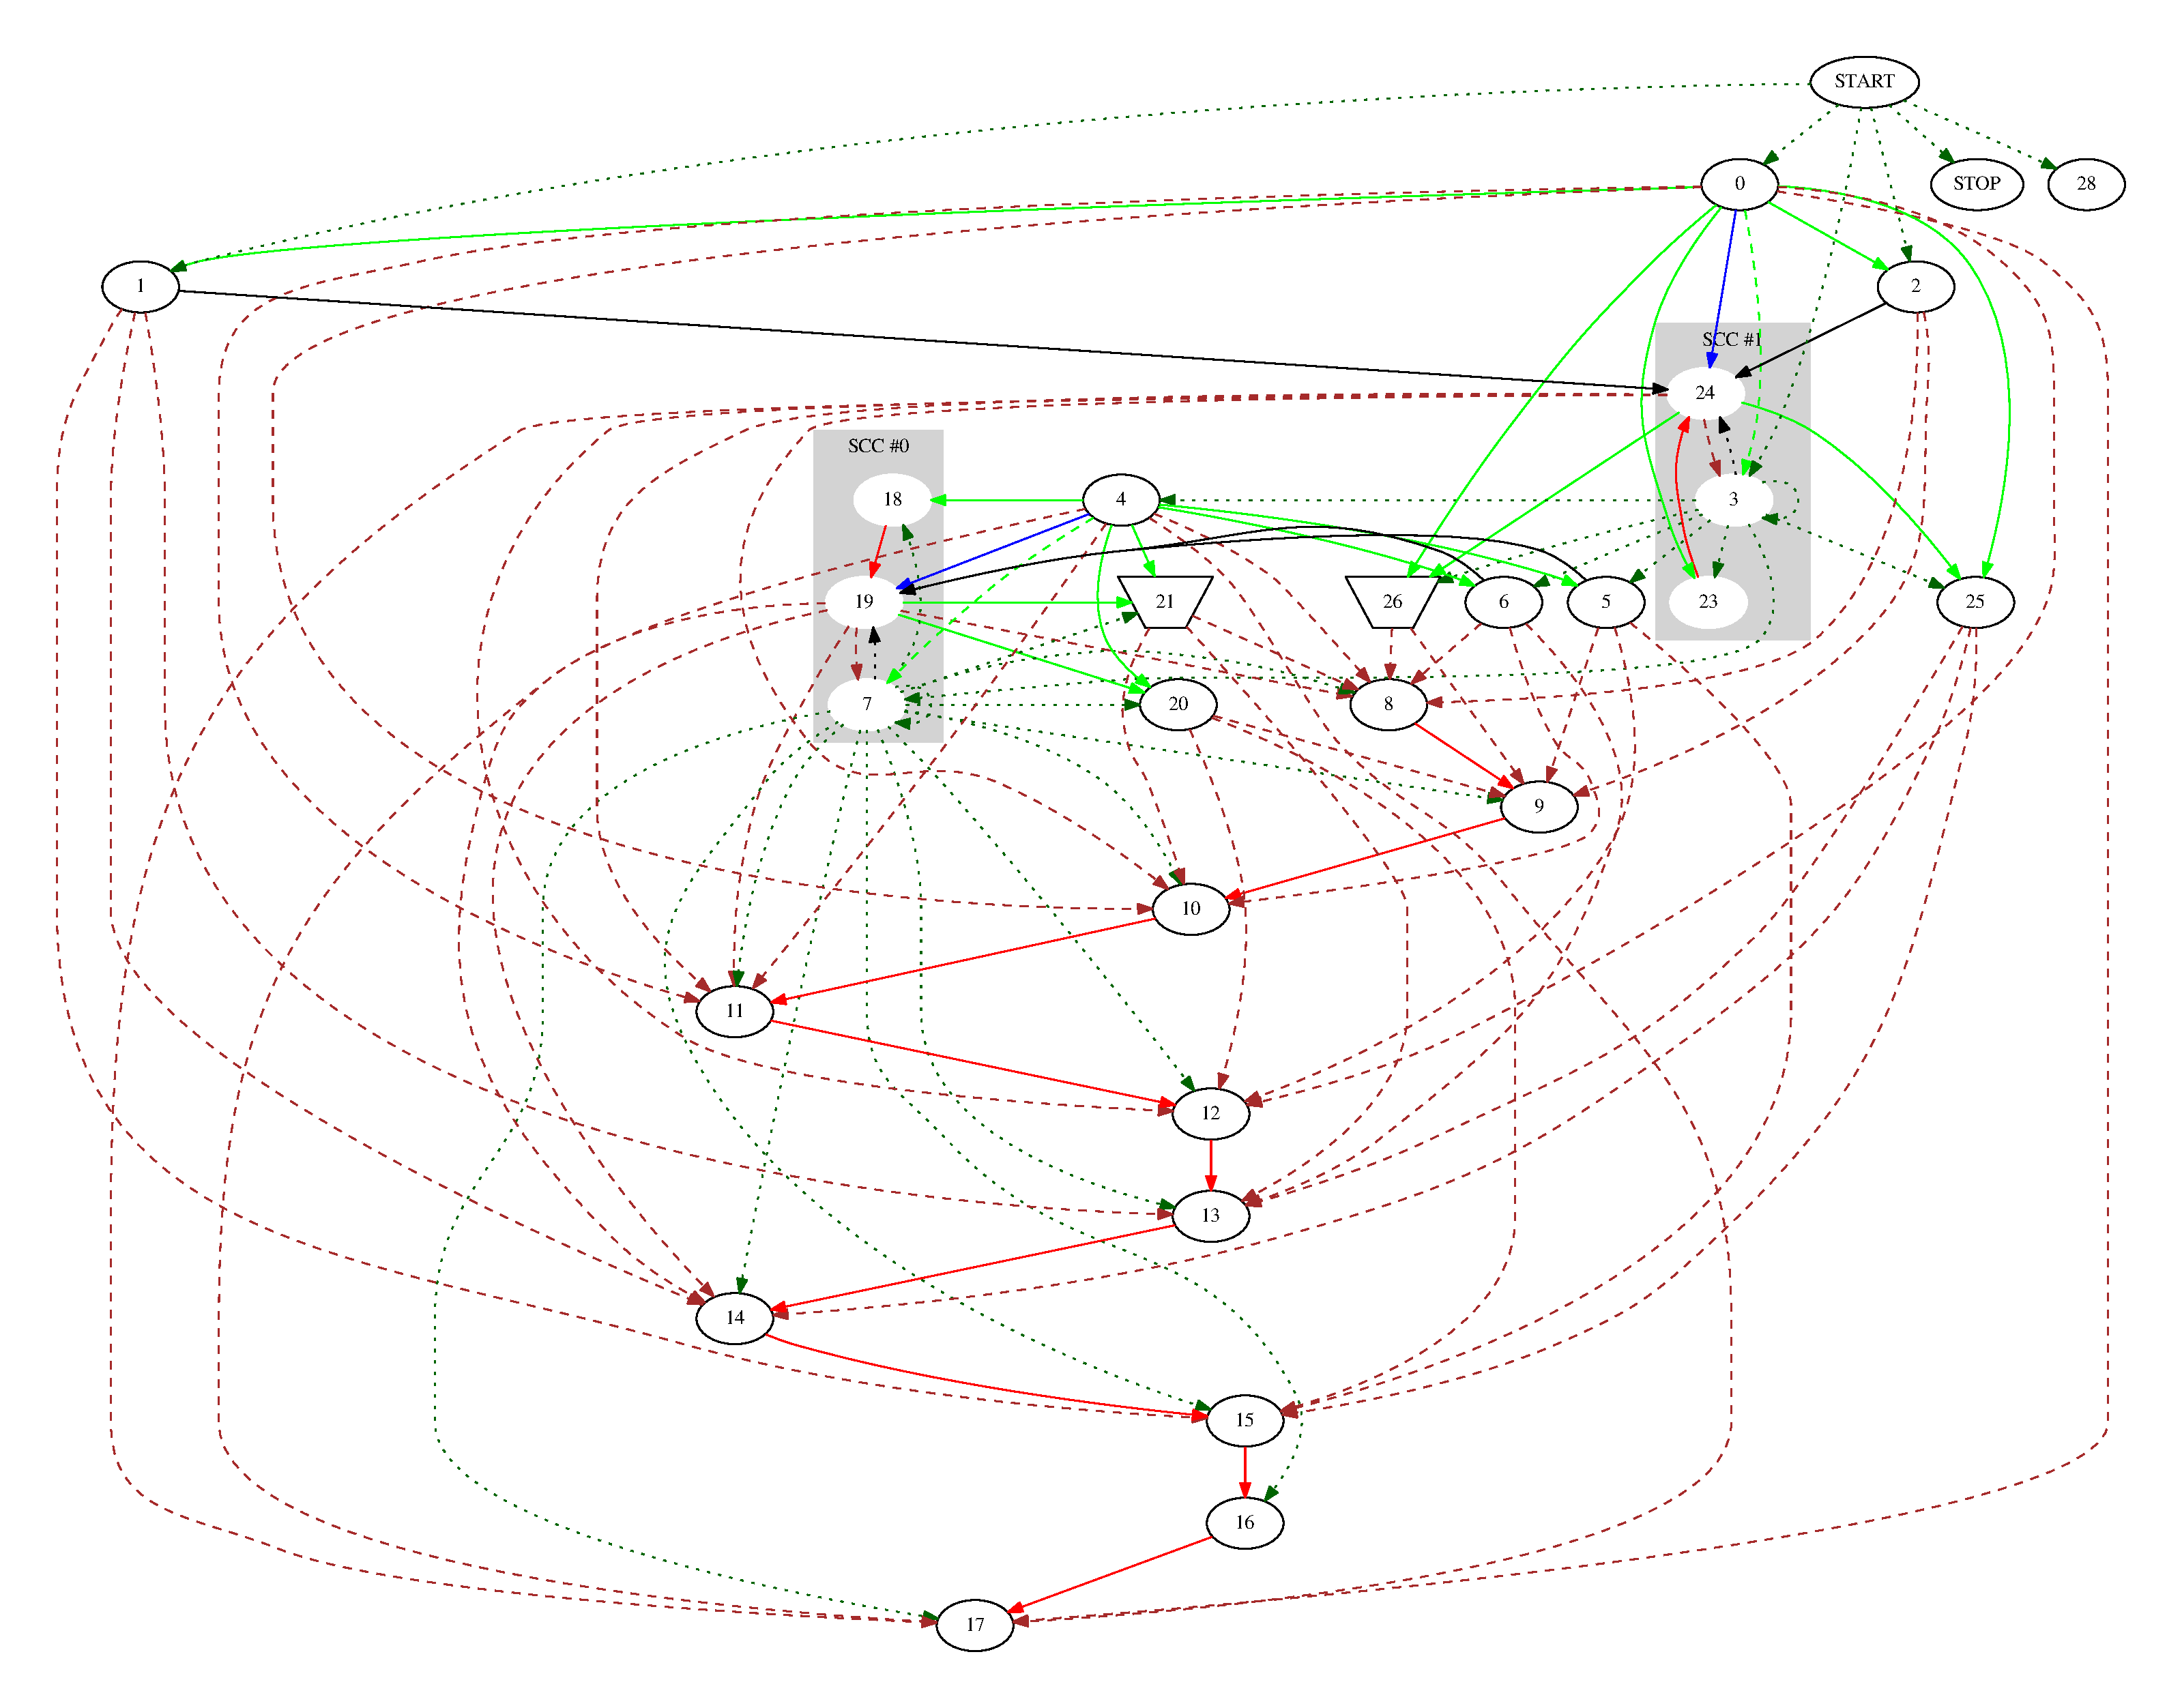
\includegraphics[width=\textwidth]{imm/tessa/PDGscc.pdf} 	\caption{Program Dependence Graph (PDG) of the Binomial Filter's MIRcode
  	} 
  	\label{pdg}
  \end{figure}
  \clearpage
  \subsubsection{Quotient Graph (Q) and topological sort}
  
 
  Quotient Graph (Q) is just the same graph PDG but with the SCCs components collapsed into a unique node. 
  \begin{figure}[h!]
  	\centering
  	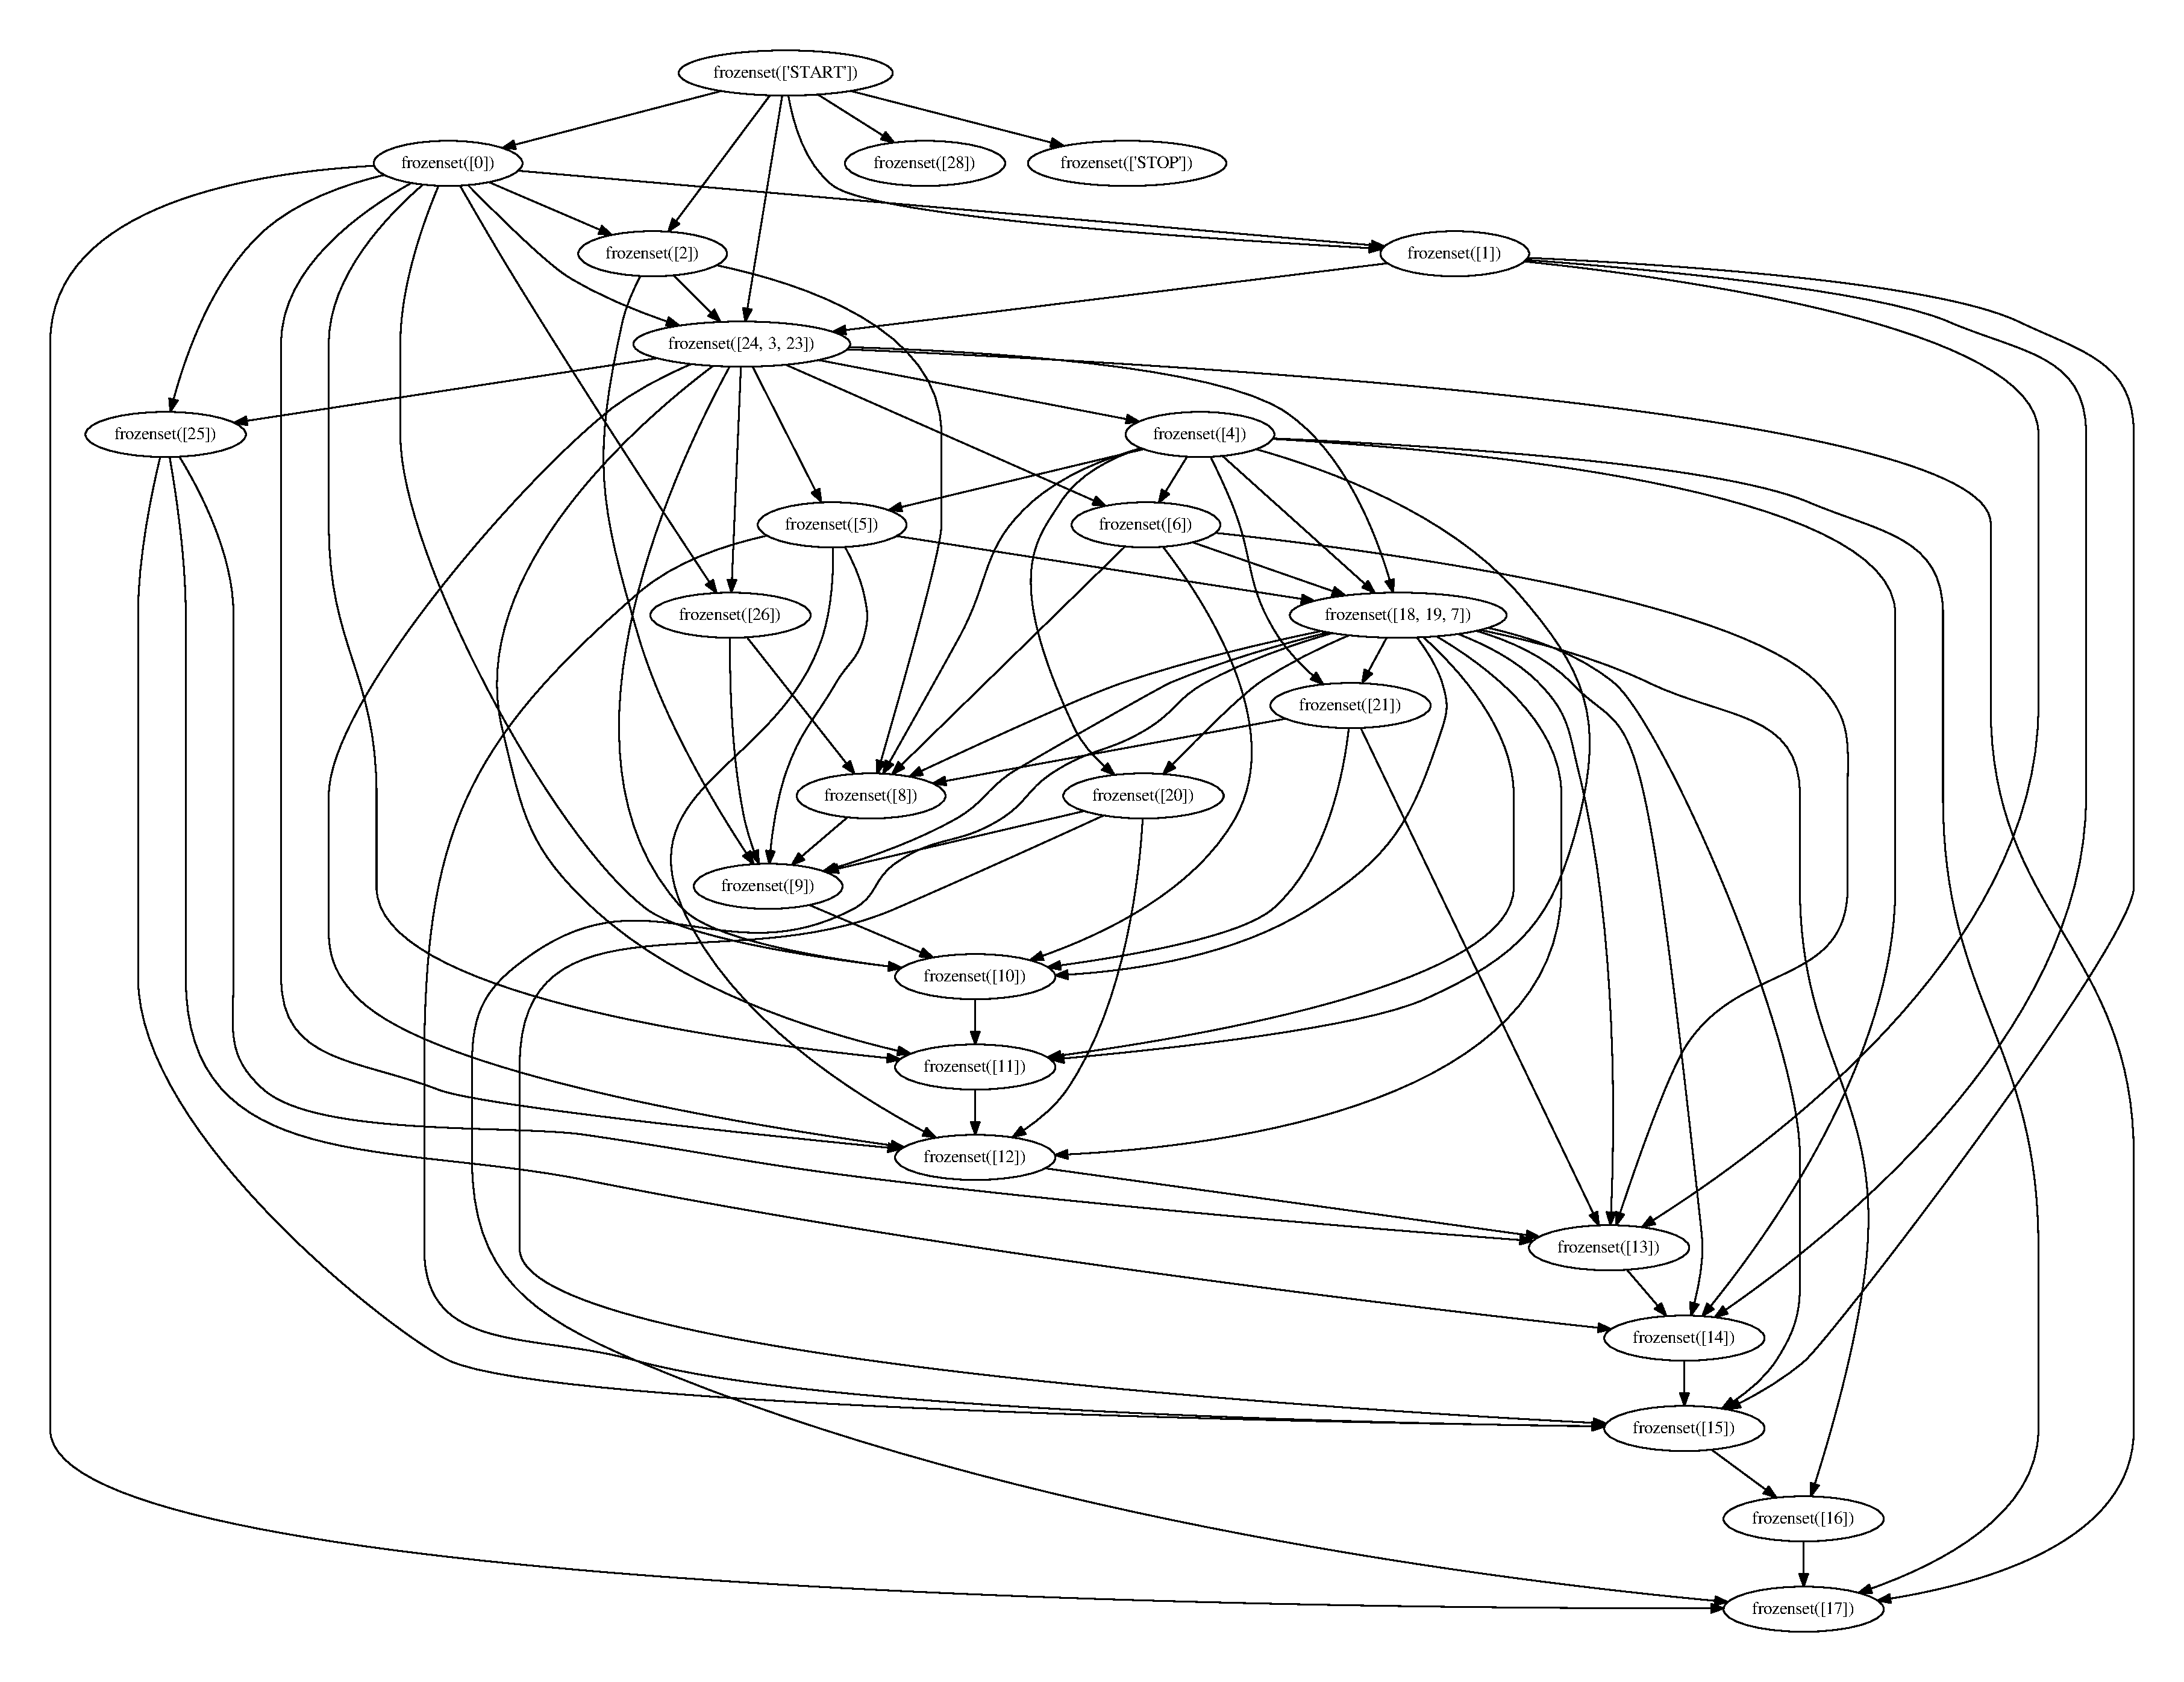
\includegraphics[width=\textwidth]{imm/tessa/Q.pdf} 	\caption{Quotient Graph Q of the Binomial Filter's MIRcode
  	} 
  	\label{q}
  \end{figure}
   This graph allows us to run a topological sort.\\
     The topological sort can be defined as a linear ordering of the vertexes of a directed acyclic graph (DAG). In general can be done only if the graph has no cycle inside, if there are some cycles (in general each SCCs correspond to a cycle) we can generate the quotient graph (Q) and then use the topological sort on this graph.
  
   \begin{figure}[h!]
   	\centering
   	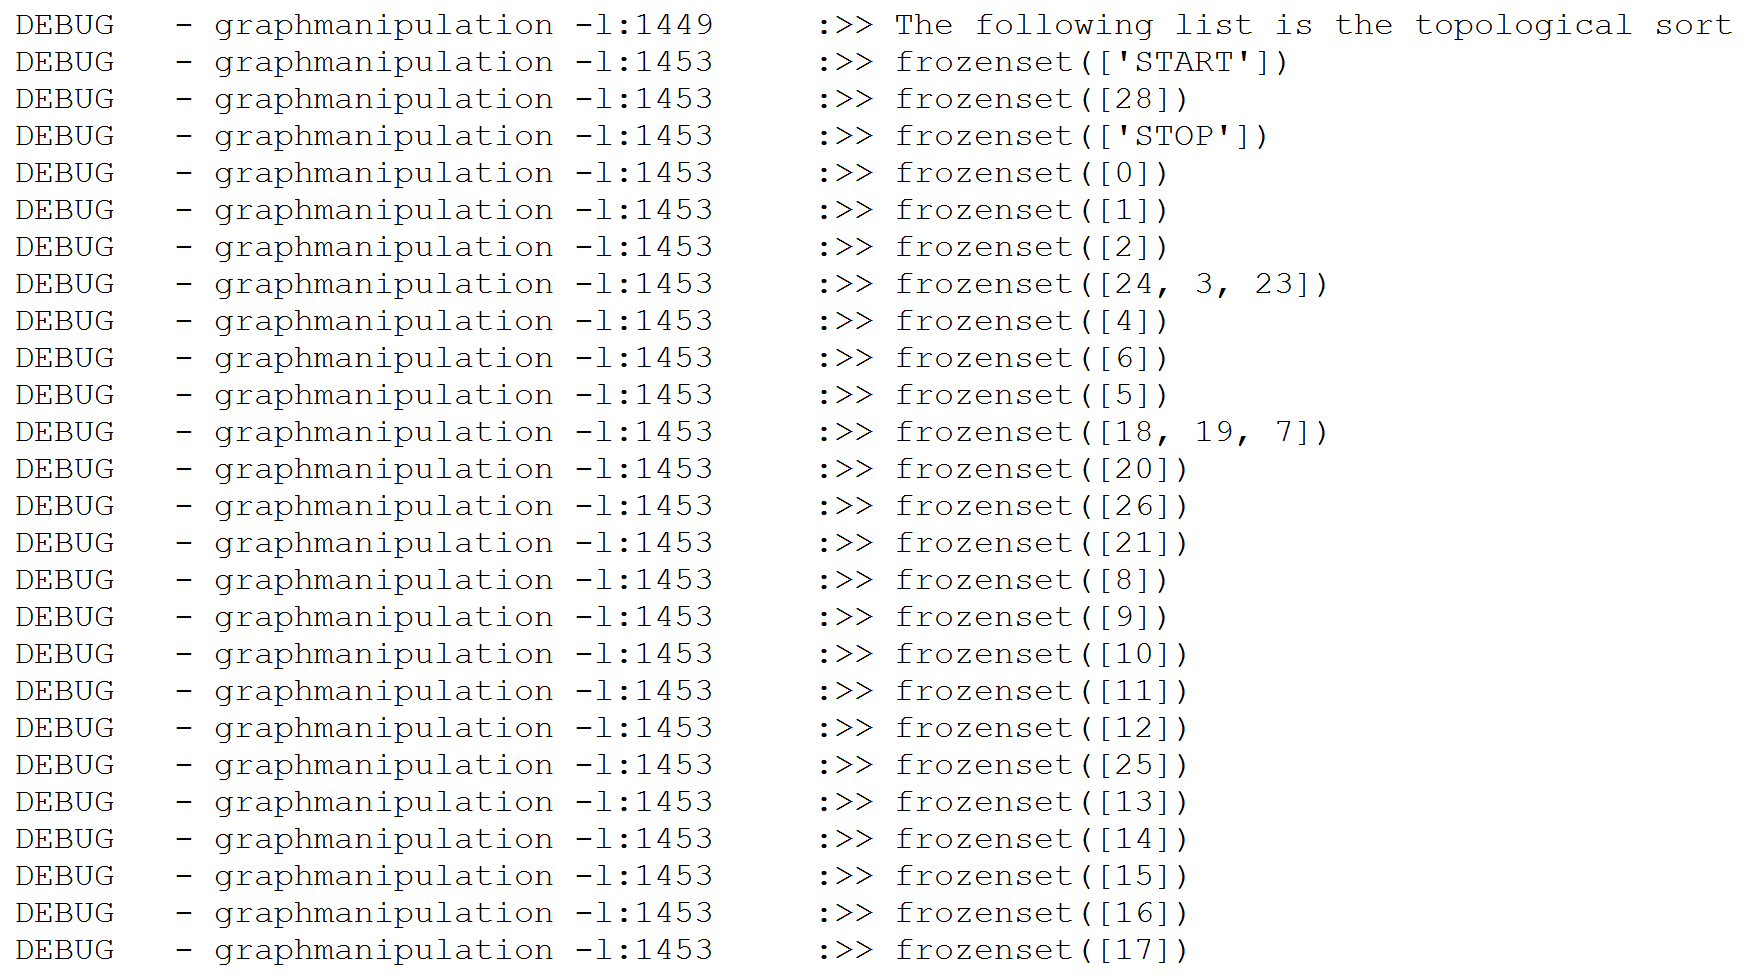
\includegraphics[width=\textwidth]{imm/tessa/topsort.png} 	\caption{Topological sort of the Binomial Filter's MIRcode
   	} 
   	\label{topsort}
   \end{figure} 
   \clearpage
  \subsection{Code Generation hints}
The instruction in the SCC (Strongly Connected Components), shown as gray box, have to be performed sequentially in the same core, while the instructions linked in red lines (strong data dependencies) have can be performed sequentially in pipeline. The instructions in dot red line shows a weak data dependencies.\\


\textit{The topological sort doesn't give the best solution, but what it gives is always correct (with respect to the correct starting graph).} \\

\textit{ Only the nodes that are inside the loop are relevant for the optimization. This because the nodes that don't need to be executed multiple time because they are inside a for can be are not liked in particular to as specific core, but can used and merged to other one, }

\section{How to use}
\subsection{Install python 2.7}
To install python 2.7.13 you can see this  \href{https://tecadmin.net/install-python-2-7-on-ubuntu-and-linuxmint/#}{website}
It is adviced to install these prerequisites before installing Python
\begin{lstlisting}[language=bash]
	$ sudo apt-get update
	$ sudo apt-get install build-essential checkinstall
	$ sudo apt-get install libreadline-gplv2-dev libncursesw5-dev libssl-dev libsqlite3-dev tk-dev libgdbm-dev libc6-dev libbz2-dev
\end{lstlisting}


download and extract the package (if you cannot download it normally, open the package and then extract it manually)
\begin{lstlisting}[language=bash]
$ cd /usr/src
$ wget https://www.python.org/ftp/python/2.7.13/Python-2.7.13.tgz
$ tar xzf Python-2.7.13.tgz
\end{lstlisting}



compile python source
\begin{lstlisting}[language=bash]
$ cd Python-2.7.13
$ sudo ./configure
$ sudo make altinstall
\end{lstlisting}

to see which version of python you have, open the terminal and digit\\
\begin{lstlisting}[language=bash]
\$ python2 --version
\end{lstlisting}


\subsection{PIP (Python package manager) and setuptools}
First, make sure you have the lastest version of pip (Python package manager) installed.
if you do not, digit the following lines\\
\begin{lstlisting}[language=bash]
$ sudo apt install python-pip
$ pip install --upgrade pip
\end{lstlisting}

Before installing networkx, you need the setuptools\\
\begin{lstlisting}[language=bash]
\$sudo apt-get install python-setuptools
\end{lstlisting}

\subsection{networkx}
Now you can try to install networkx\\
\begin{lstlisting}[language=bash]
\$ pip install networkx
\end{lstlisting}


If you do not have permission to install software systemwide, you can install into your user directory using the "--user" flag:\\
\begin{lstlisting}[language=bash]
$ pip install --user networkx
\end{lstlisting}

\subsection{Graphviz}
Now you need to install \textit{Graphviz}, an open source graph visualization software and other things:\\
\begin{lstlisting}[language=bash]
$sudo apt-get install graphviz
\end{lstlisting}


\subsection{Running Tessa tool}
You can run the tessa tool.
Open the terminal and go to the folder "\textit{graphelab}" and run the bash script\\
\begin{lstlisting}[language=bash]
$ bash run\_tool.sh
\end{lstlisting}


A list of all the C codes (in the folder "\textit{modules/class/test}") will appear.\\
You have to digit the C file you want to analyze
	\begin{figure}[h]
		\centering
		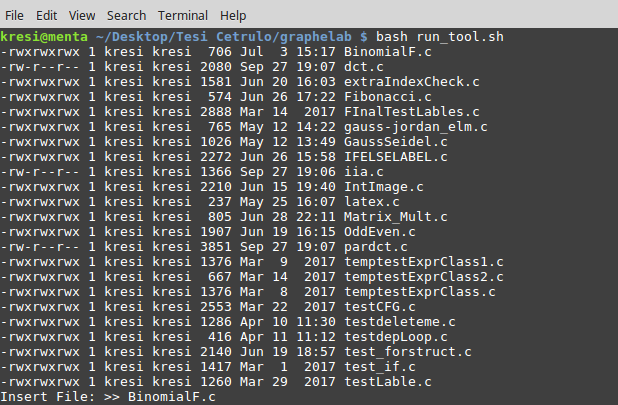
\includegraphics[width=\textwidth]{imm/tessa/list_C.png}  
		\caption{List of all your C files}
		\label{listC}
	\end{figure}
If you get the error:\\
\textit{ImportError: No module named pylab}\\
Is probably because you need some packages which provide additional functionality:
\begin{itemize}
	\item \textbf{NumPy} provides matrix representation of
	graphs and is used in some graph algorithms for high-performance matrix
	computations.
	\item \textbf{SciPy} provides sparse matrix representation
	of graphs and many numerical scientific tools.
	\item \textbf{pandas} provides a DataFrame, which
	is a tabular data structure with labeled axes.
	\item \textbf{Matplotlib} provides flexible drawing of
	graphs.
	\item \textbf{PyGraphviz} and \textbf{pydot} provide graph drawing
	and graph layout algorithms via \textit{GraphViz}.
	\item \textbf{PyYAML} provides YAML format reading and writing.
	\item\textbf{ gdal} provides shapefile format reading and writing.
	\item \textbf{lxml} used for GraphML XML format.
\end{itemize}
Since I keep getting some errors, i decided to install all the packages.\\
To install \textit{networkx} and all optional packages, do:\\
\begin{lstlisting}[language=bash]
$ pip install networkx[all]
\end{lstlisting}

To explicitly install all optional packages, do:
\begin{lstlisting}[language=bash]
$ pip install numpy scipy pandas matplotlib pygraphviz pydot pyyaml gdal
\end{lstlisting}



If you get the error:\\
\textit{gnome-open: command not found}\\ 
\begin{lstlisting}[language=bash]
\$sudo apt-get install libgnome2-0
\end{lstlisting}

Now this is where my exploration on tessa tools ends.
I get the error:\\
\textit{TypeError: 'OutEdgeDataView' object does not support indexing} 	
\begin{figure}[h]
	\centering
	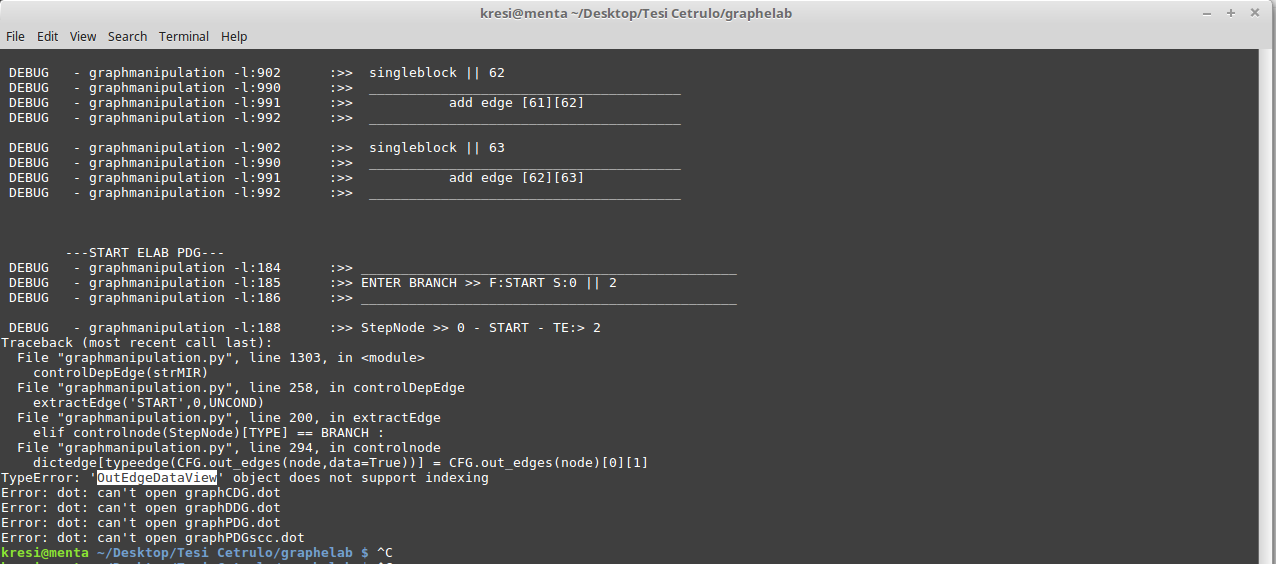
\includegraphics[width=\textwidth]{imm/tessa/OutEdgeDataView.png}  
	\caption{OutEdgeDataView}
	\label{OutEdgeDataView}
\end{figure}
I tried to find where the object 'OutEdgeDataView' was declared but I didn't find it on the script. Then, after searching on internet, I figure it out it was written in the file "\textit{reportviews.py}" which was in the folder "\textit{~/.local/lib/python2.7/site-packages/networkx/classes}"
And without this script, i can't get the graphs
\begin{lstlisting}[language=bash]
\end{lstlisting}
Toy Parser Generator\\
http://cdsoft.fr/tpg/\\
go to the folder "TPG-3.2.2" and run\\
python setup.py install

https://networkx.github.io/

http://www.graphviz.org/  
run the bash script

place your c file in the folder modules/class/test